\chapter{Background}\label{ch2:background}

\section{Geothermal Systems}\label{ch2:geosys}
\subsection{Heat Origins}\label{ch2:heatorig}
\subsubsection{Accretion}\label{ch2:accrete}
The story of geothermal energy begins with the birth of planet Earth. Approximately 4.56 billion years ago \citep{allegre_age_1995, patterson_age_1956}, the Earth coalesced as a molten body heated by repeated impacts with other objects in the early solar system, like the planetesimal collision responsible for the formation of the Moon \citep{stevenson_origin_2014}. Over tens of millions of years, the Earth compacted, cooled, and differentiated, settling into the now familiar layered structure of a solid inner core, liquid outer core, viscous mantle, and outermost brittle crust \citep[~p. 7]{press_understanding_2004}. \textbf{DIAGRAM OF EARTH STRUCTURE} The intense heat from that early accretionary history remains concentrated in the core, where temperatures --- a matter of continued scientific inquiry --- fall in the range of $6000\pm500$ K \citep[~p. 372]{fowler_solid_2005}. Present day heat flux estimates for the whole Earth amount to 87 mW/m$^2$, $\sim$60\% of which flows through conductive and convective pathways from the deep interior to outermost crust \citep{stein_heat_1995}. Diffuse conductive heat transfer occurs everywhere across of the Earth’s surface, but heat flow concentrates along tectonic plate boundaries. In fact, the subduction-sourced volcanoes that ring the Pacific Ocean, divergent zones at the mid-ocean ridges and East African rift, and major strike-slip boundaries like the San Andreas fault zone all mark locations where focused heat anomalies are already being tapped by geothermal installations \citep[~p. 16]{dipippo_geothermal_2012}.

\subsubsection{Radioactive Decay}\label{ch2:radio}
The second major source of heat within the Earth is the decay of radioactive isotopes. Early radioactive heating included radioisotopes with short half-lives like Aluminum-26 and Hafnium-182, which are now no longer present \citep[~p. 16]{glassley_geothermal_2015}. Among the radioactive elements most influential to crustal heat  today are uranium (U), thorium (Th), rubidium (Rb), and potassium (K) \citep[~p. 17]{glassley_geothermal_2015}. The decay of these and other elements accounts for 40\% of the crustal thermal budget \citep{stein_heat_1995}. But element abundances are not distributed uniformly throughout the crust. On average, continental crust, particularly the upper continental crust, has significantly higher concentrations of U, Th, and K radioactive elements compared to oceanic crust, and both types of crust are 1-2 orders of magnitude more enriched than the mantle \citep[~p. 276]{fowler_solid_2005}. This relationship holds for representative igneous rock types; granite generates more heat than basalt, and both out-produce ultramafic rocks like peridotites \citep[~p. 276]{fowler_solid_2005}.

\subsection{Heat Measurements}\label{ch2:heatmeas}
\subsubsection{Geothermal Gradient}\label{ch2:geotherm}
Average subsurface conditions show a steady increase in temperature with depth, commonly referred to as the geothermal gradient, sustained by the flow of original accretionary heat and generated radioactive heat. On average, the gradient for continental crust is $\sim30^\circ$C/km \citep[~p. 209]{press_understanding_2004}. However, deviations from this value are common and reflect the complexity of the rock record in an area. The crust comprises a distinct set of layers, or strata, that vary in composition and rock type. Unlike the aforementioned igneous formations that can be relatively homogeneous, surface processes mix sediments from a variety of original source rocks, sometimes sorting them well and sometimes not, before they get deposited and indurated into sedimentary formations \citep[~p. 164-168]{press_understanding_2004}. Alteration from fluids, heat, and pressure can then modify the composition of these rocks, causing constituent minerals to change form and arrangement to create metamorphic rocks \citep[~p. 195-205]{press_understanding_2004}. The spatial and depth variations in these formations create subsurface compositional heterogeneity, directly reflected in rock properties. Thermal conductivity, specifically the ability to move deep-sourced heat to shallower depths, and radioactive element abundance, or the ability to generate additional heat in situ, can therefore vary in all directions in the subsurface. Thermal heterogeneity can be further compounded by anomalies created from salt movement \citep[~p. 164-168]{press_understanding_2004}, magmatic intrusions, or global tectonic processes. Geology and geologic history therefore play an important role in defining the geothermal gradient of an area.

\subsubsection{Heat Flow}\label{ch2:heatflow}
Fundamentally, heat moves in the direction from hot to cold (Second Law of Thermodynamics) at a rate that linearly scales with the thermal gradient. Simple, one-dimensional thermal conduction can be characterized by the relationship \citep[~p. 270]{fowler_solid_2005}:
\begin{equation}\label{eq:conduction}
q = -k \frac{\nabla T}{x}
\end{equation}
where q is heat flux, or heat flow per unit time per unit area, with S.I. units of Wm$^{-2}$. Heat flux depends on the gradient of temperature (T), the distance over which conduction takes place (x), and the thermal conductivity (k), that is, the ability of material to conduct heat. Different rock types have different values of k, e.g., sandstone varies from 1.60-2.10 W/m$^\circ$C while granite tends to be higher with values ranging from 1.73-3.98 W/m$^\circ$C \citep[~p. 30]{dipippo_geothermal_2012}. Feldspars and quartz exhibit significant (up to 3x) differences in k values. As the most abundant minerals in crustal rocks, their relative fractions will strongly influence the thermal conductivity of a formation \citep[~p. 22]{glassley_geothermal_2015}. Regardless, typical crustal minerals tend to be relatively poor thermal conductors compared to metals like aluminum (210 W/m$^\circ$C) and iron (73 W/m$^\circ$C), making conduction a slow method of crustal heat transmission \citep[~p. 23]{dipippo_geothermal_2012}.

Conduction dominates on local scales in the crust, while convection is the primary means of heat transfer on global, tectonic scales. Even in its two-dimensional form with no internal heat generation, the equation governing convection is much more complex than for conduction \citep[~p. 355]{lowrie_fundamentals_2007}:
\begin{equation}\label{eq:convection}
\frac{\partial T}{\partial t} = \left (\frac{k}{\rho * c_P}\right)\left (\frac{\partial ^2T}{\partial x^2}+\frac{\partial ^2T}{\partial z^2}\right)-u_x\frac{\partial T}{\partial x}-u_z\frac{\partial T}{\partial z}
\end{equation}
where \textbf{u} = ($u_x$, $u_z$) is the velocity of the fluid, $\rho$ is the material density, and $c_P$ is the specific heat, which defines the amount of heat necessary to raise 1 kg of that material by $1^\circ$C Convention combines heat transfer from conduction with mass movement. Since the minerals are relatively poor conductors of heat, the combined effects of lower viscosity and thermal expansion --– as seen near the core-mantle boundary –-- and gravitational forces that create buoyancy effects, all create the right conditions for convective flow, e.g., within the mantle \citep[~p. 25]{glassley_geothermal_2015}. Mantle convection is responsible for the high heat flow values observed at crustal plate boundaries like mid-ocean ridges, as well as intraplate diapiric hot spots underlying Hawaii, Yellowstone, and a number of other locations around the world. Smaller-scale convection also takes place at subduction zones where the material from the down-diving plate melts at lower temperatures with the presence of water, migrates upwards, and forms volcanic arcs on the surface as observed in Japan, Indonesia, and the Pacific Northwest of the U.S. \citep[~p. 31-33]{press_understanding_2004} --– all locations with geothermal potential.

Heat flow measurements capture the flux of heat through the Earth’s surface as a result of these and other complex processes taking place in the subsurface. In this respect, it serves as a simpler and more accessible metric for local or regional heat potential than the more sparsely-measured and less well-constrained geothermal gradient. Today, high-quality heat flow measurements can be obtained in marine conditions, on continental margins, on mid-ocean ridges, and from the multitude wells drilled by the oil \& gas industry, supporting the creation of large heat flow data sets like the New Global Heat Flow Database \citep{lucazeau_analysis_2019}. As Figure \ref{fig:heatflow} shows, data from these collections can be gridded to create spectacular maps of heat flow variations around the world. These maps offer a good starting point for quickly targeting where the greatest geothermal potential exists at the regional scale, which can then be further refined through additional methods (see Section \ref{ch2:geoexp}).
\begin{figure}[h!]
\centering
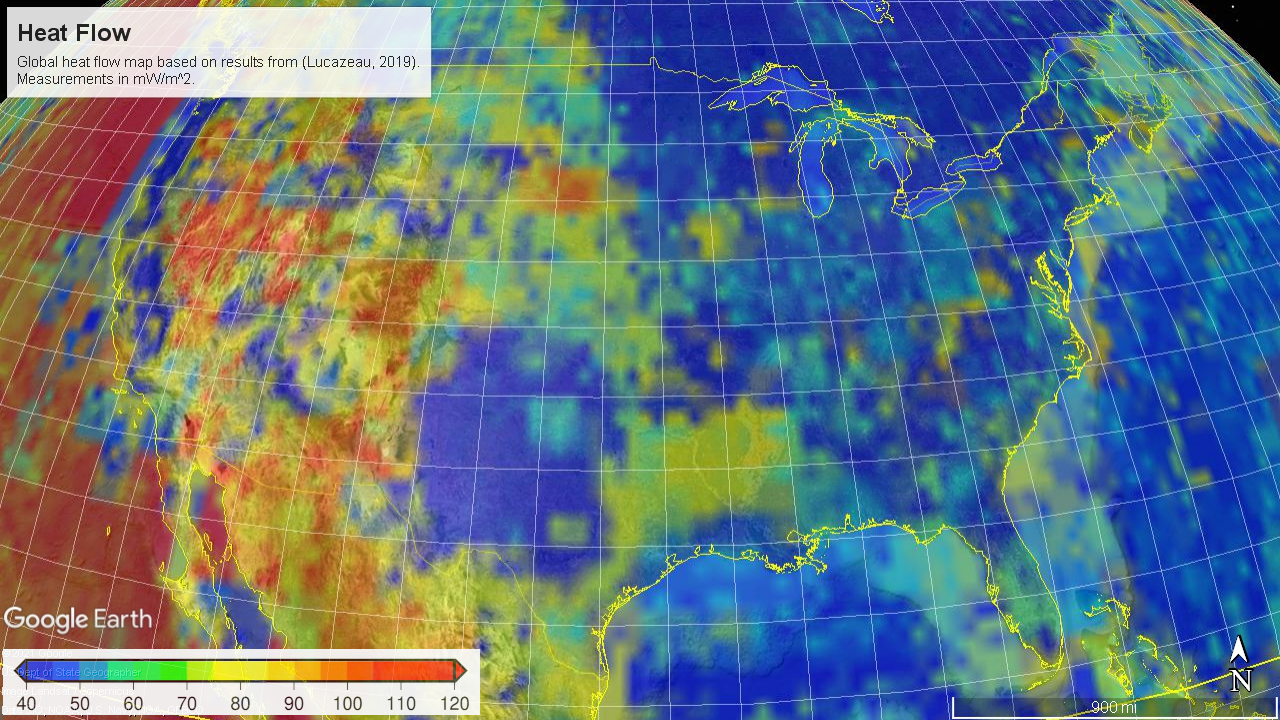
\includegraphics[scale=0.45]{Figure-HeatFlowMap}
\caption[Heat flow across the continental U.S.]{Heat flow estimates for the continental United States, plotted in Google Earth with data layer from \protect\citep{lucazeau_analysis_2019}}
\label{fig:heatflow}
\end{figure}

\subsection{System Fundamentals}\label{ch2:sysfund}
The conventional concept of a geothermal system consists of five key entities \citep[~p. 9]{dipippo_geothermal_2012}:
\renewcommand{\labelenumi}{\roman{enumi}}
\begin{enumerate}\label{list:sysreq}
   \item Heat source of significant size and temperature
   \item Permeability, typically in the form of a fracture network within crystalline rock
   \item Ample volume of working fluids, e.g. water from precipitation and drainage
   \item Impermeable sealing layer
   \item Consistent, reliable fluid recharge
\end{enumerate}

\subsubsection{Hydrothermal Systems}\label{ch2:hydro}
If naturally present, the combination of these five elements defines a hydrothermal system. As water percolates down, captures heat from the permeable thermal reservoir, and gets trapped beneath the sealing caprock, a small fraction of the resource can escape to the surface to produce distinctive geothermal manifestations like fumaroles, hot pools, geysers, mud pots, and discolored or altered rocks (Figures \ref{fig:lassen-geysers} and \ref{fig:lassen-mudpot}). These features are strong indicators of hydrothermal resources at depth.
\begin{figure}[h!]
\centering
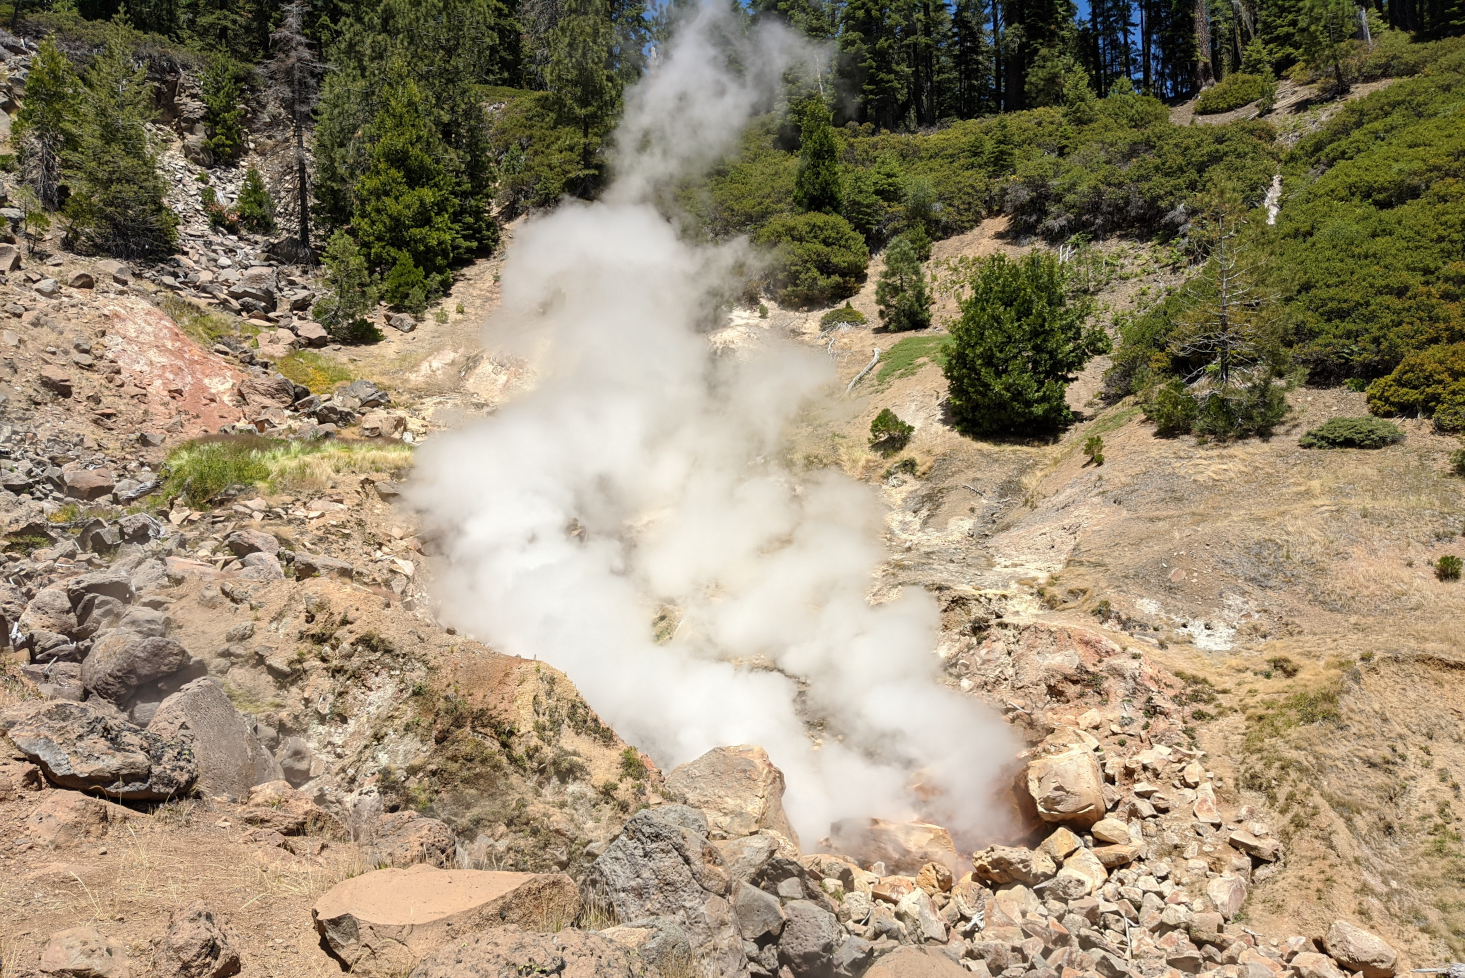
\includegraphics[scale=.84]{Figure-Lassen-geysers3}
\caption[Terminal Geyser, Lassen National Park]{Terminal Geyser, Lassen National Park, California. Photo credit: Author}
\label{fig:lassen-geysers}
\end{figure}
\begin{figure}[htbp]
\centering
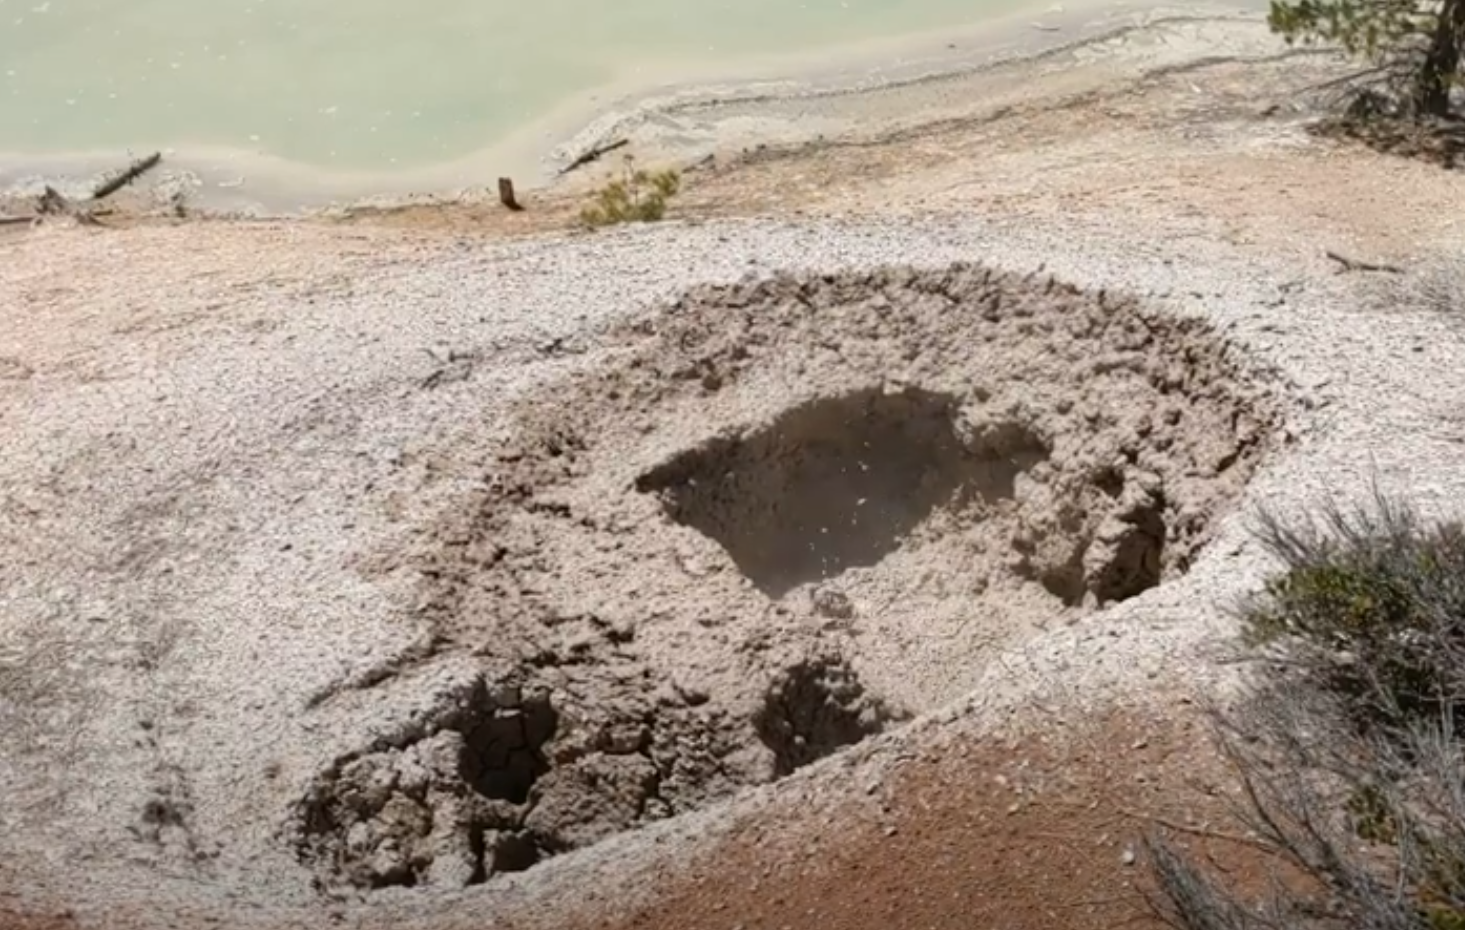
\includegraphics[scale=0.27]{Figure-Lassen-mudpot}
\caption[Mud pot, Lassen National Park]{Active mud pot and ground staining on the bank of Boiling Springs Lake, Lassen National Park, California. Photo credit: Author}
\label{fig:lassen-mudpot}
\end{figure}

Hydrothermal resources have been exploited by humans for many millennia. Artifacts show proto-Native American use of hydrothermal waters for cleaning and health restoration over 10,000 years ago \citep{doe_history_2021}. The importance of geothermal hot springs for Roman, Japanese, Chinese, and Ottoman baths is also well-established in the historical record \citep{lund_characteristics_2007}. Industrial use began in the 1800s with chemical extraction from geothermal steam, pools, and deposits in Larderello, Italy \citep[~p. 251]{dipippo_geothermal_2012}. \acrlong{gdh} (\acrshort{gdh}), or large-scale heating of residences and businesses using geothermal-produced fluids, was pioneered in Chaudes-Aigues, France in the 1300s and first introduced to the United States in 1892 with an installation in Boise, Idaho \citep{lund_characteristics_2007}.

These few examples show some of the many potential opportunities for low-temperature ($<90^\circ$C) and medium-temperature ($<150^\circ$C) geothermal resource use, even beyond hydrothermal systems. GDH can help meet building and water temperature needs, and agriculture, textiles, chemicals, and even the food industry can benefit from access to low-temperature geothermal resources \citep{doe_low_2021, liu_overview_2015}. Growing interest has led to dedicated funding opportunities from agencies like the \acrlong{gto} (\acrshort{gto}) within the \acrlong{doe} (\acrshort{doe}); a grant recently awarded to Cornell University supports piloting a deep direct-use geothermal project to provide baseload heating for the university campus supporting peak demand during cold upstate New York winter months  \citep{hamm_geothermal_2021,tester_integrating_2015}.

The topic of this thesis instead concerns the use of moderate- to high-temperature geothermal for power generation. The first example of geothermal power production came from Italian experiments in 1904, and the first commercial plant went online in Larderello, Italy in 1914 \citep[~p. 251]{dipippo_geothermal_2012}. Geothermal-generated electricity made its debut in the United States with the development of The Geysers field beginning in 1960 \citep{tester_future_2006}. Hydrothermal plants quickly appeared in New Zealand, Japan, Iceland, Indonesia, Kenya, Philippines and elsewhere throughout the 1970s-1980s, with continued growth through to present-day \citep{lund_characteristics_2007}. 2020 statistics from the \acrlong{irena} (\acrshort{irena}) place the United States as world leader in geothermal installed capacity (2587 MWe), followed by Indonesia (2131 MWe) and Philippines (1928 MWe) \citep{irena_country_2021} (Figure \ref{fig:irena-rank}). 

\begin{figure}[htbp]
\centering
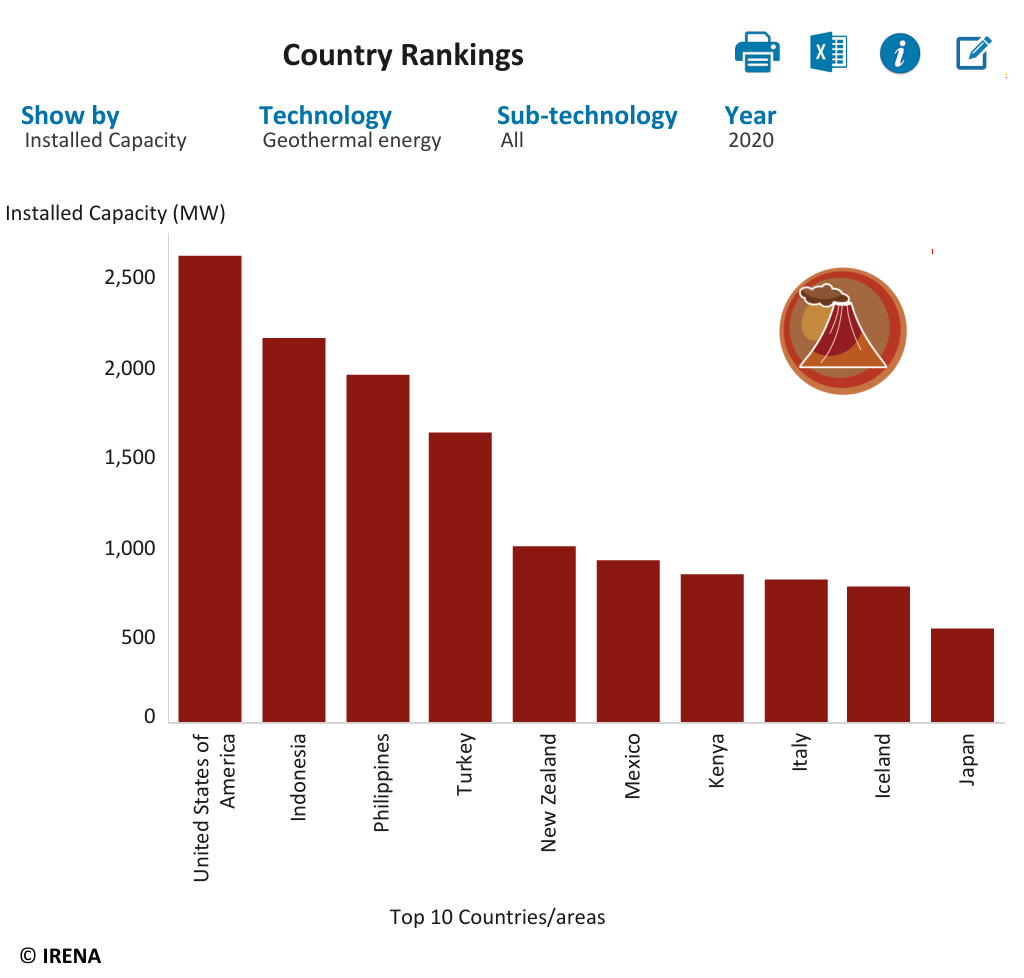
\includegraphics[scale=.45]{Figure-IRENA_Rankings}
\caption[Country rankings, installed geothermal capacity ]{Countries ranked by installed geothermal capacity, from \protect\citep{irena_country_2021}}
\label{fig:irena-rank}
\end{figure}

A comprehensive assessment of moderate and high-temperature \acrlong{kgra}s (\acrshort{kgra}s) by the \acrlong{usgs} (\acrshort{usgs}) determined the U.S. has conventional geothermal (hydrothermal) power generation potential of $\sim$9,000 MWe, and an additional $\sim$30,000 MWe potential exists in undiscovered resources \citep{williams_assessment_2008}. The recent DOE GeoVision study notes hydrothermal potential in Alaska and Hawaii alone are $\sim$8000 MWe due to their unique tectonic environments (Aleutian subduction zone and Hawaiian hot spot, respectively), and high-case model estimates for the continental U.S. forecast an installed capacity of $\sim$16.5 GW by 2050 for known and unknown hydrothermal resources \citep{augustine_geovision_2019,hamm_overview_2019}.

\subsubsection{Enhanced Geothermal Systems}\label{ch2:egs}
In some cases, the potential for a geothermal system exists even when one or more of the fundamental elements listed in Section \ref{ch2:sysfund} are missing. These unconventional geothermal systems, often referred to as \acrlong{egs} (\acrshort{egs}), contain a significant heat source but lack either the adequate permeability or sufficient rechargeable working fluids to meet the requirements of a hydrothermal system. A broader definition for EGS includes thermal production from sedimentary and crystalline tight rock, poorly-performing hydrothermal systems, co-production from oil \& gas operations, and even thermal recovery directly from magma \citep{tester_future_2006}. Focusing on the more common tight rock scenario, EGS systems work by artificially creating or improving reservoir permeability and ensuring sustained flow rates of fluids through the reservoir \citep[~p. 281]{glassley_geothermal_2015}. Fluids pumped down an injection well pass through a stimulated fracture network, heat up through direct contact with the thermal reservoir, and return to the surface via one or more producing wells to serve as inlet fluids for a power plant \textbf{DIAGRAM OF EGS}. Reservoir stimulation generally involves hydraulic fracturing (hydro-fracking or just “fracking”) techniques to create pathways connecting injector-producer pairs. The associated technology and capabilities are thus well-aligned with unconventional oil \& gas operations \citep{petty_synergies_2009}. 

EGS can provide the bridge between geothermal use in niche hydrothermal environments and a more comprehensive adoption of geothermal energy for electricity generation across the United States. The sources of subsurface heat (see Section \ref{ch2:heatorig}) exist everywhere, so accessing a range of temperatures that could support power production relies on drilling deep enough and creating the artificial conditions necessary for heat capture. \acrlong{lanl} (\acrshort{lanl}) validated the EGS approach in crystalline rock at Fenton Hill beginning in 1974. Feasibility studies followed soon thereafter in Japan, Germany, the U.K., and France \citep{breede_systematic_2013}. Among the most notable EGS projects that provided key lessons learned are The Geysers (U.S), Soultz-sous-Forêts (France), and Cooper Basin (Australia). The Geysers stands out as the largest geothermal power-generating complex in the world, providing $\sim$1,000 MWe for California even after 60 years of steam production \citep{jelacic_evaluation_2008,williams_assessment_2008}. Although drilling issues and public concern over induced seismicity halted efforts \citep{manish03_united_2009}, rock stimulation experiments in the Northwest Geysers proved distinct reservoirs can be developed adjacent to active hydrothermal operations \citep{pan_establishment_2019}. The Soultz project commenced in 1987 with one injector and two producers drilled to 5 km depth to support a 1.5 MW power plant built in 2007-2008 \citep[~p. 463]{dipippo_geothermal_2012}. In addition to many experimental lessons learned around drilling, hydrofracturing, chemical stimulation, scaling and corrosion, Soultz today supports both electricity production and direct-use district heating \citep{durst_overview_2013}. Cooper Basin, the largest EGS demonstration project in the world, showed great promise after a 6-year proof of concept phase \citep{stephens_assessing_2010}. However, the project halted in 2015 due poor stimulation results tied to an unrecognized fault, highlighting the importance of robust structural appraisal in assessing geothermal prospects \citep{holl_what_2015}. 

As the fate of these projects might suggest, the long-standing promise of EGS has not yet been fully realized. However, several active projects supported by the \acrlong{nrel} (\acrshort{nrel}) and the DOE (e.g. EDGE, FORGE, EGS Collab) are providing the insights necessary to mature subsurface models, drilling technologies, and stimulation methods for more widespread EGS adoption \citep{hamm_geothermal_2021}. And recent technology advances and partnerships involving start-ups Fervo Energy \citep{moss_google_2021,shieber_geothermal_2021}, Deep Earth Energy \citep{geoenergy_saskatchewan_2021}, Eavor Technologies \citep{ross_energy_2020}, and Climeon \citep{climeon_climeon_2021,geoenergy_baseload_2020} show there is a growing fervor to overcome the technology roadblocks currently holding EGS back. Projections show the size of the prize with success in EGS. Assuming a maximum cut-off depth of 7 km and a minimum reservoir temperature of 150$^\circ$C, the EGS resource potential for electricity production in the continental United States might be at least 5,150 GWe, with an additional $\sim$1,500 MWe from Near Hydrothermal Field-EGS (\acrshort{nfegs}) \citep{augustine_geovision_2019}. To put this opportunity into context: the total utility-scale electricity generation capacity from \underline{all} sources in the United States was $\sim$1,200 GWe in 2019, over 4x less in magnitude than the predicted EGS potential \citep{eia_electric_2020}.

\section{Geothermal Exploration}\label{ch2:geoexp}
\subsection{Background}
Historically, the identification of geothermal resources primarily relied on surface expressions of hot fluids circulating at depth. Quite simply, if a bubbling hot spring or a geyser was present, you had a working hydrothermal system. Some of the first sites for geothermal power production, like Larderello and The Geysers, were (unsurprisingly) targeted because of their tell-tale surface characteristics \citep[~p. 111]{glassley_geothermal_2015}. However, this prospecting method only applies to fully-functioning hydrothermal systems, and not all such systems have surface manifestations if fluids remain trapped beneath a subsurface impermeable seal. These hidden or “blind” geothermal resources require more sophisticated exploration methods to identify and assess accurately.

\subsection{Regional Exploration}
Regional evaluation techniques classically relied on sparse borehole data, including water wells and oil \& gas wells, to map out the geothermal potential of the U.S. \citep{kehle_aapg_1970}. Successive efforts led to progressively more comprehensive collections of surface heat flow and borehole temperature measurements \citep{blackwell_temperature-at-depth_2011, blackwell_heat_1990, muffler_assessment_1979, sorey_low-temperature_1983, wisian_heat_1999}, now widely-available with other geothermal data through the DOE-funded \acrlong{ngds} (\acrshort{ngds}) platform \citep{anderson_national_2013}. These efforts supported a better understanding of broad trends directly tied to tectonic provinces in the United States. Subduction and transform plate boundaries in the West, combined with extension in the Basin and Range, make this area of the U.S. more susceptible to high heat flow, high geothermal gradient, and greater potential for hydrothermal system activity \citep{mariner_low-temperature_1983}. Passive margins on the Atlantic and Gulf of Mexico sides make those regions less likely to host significant hydrothermal systems, although surveys have identified sedimentary basins with elevated heat flow in the south (Louisiana-Arkansas), central (Iowa-Illinois, Nebraska-South Dakota), and eastern (Appalachians) parts of the country \citep{blackwell_geothermal_1995, sorey_low-temperature_1983}.

\subsection{Sub-regional Exploration}
Continental maps provide a super-regional view of geothermal prospectivity, but further refinement is required to progress an exploration program. Specifically, the determination of regional plays and local prospects must come before deciding where and how to develop a geothermal field, e.g., for electricity generation. Characterization activities can be decomposed into defining the magnitude and extent of four earth subsystems: structural, stratigraphic, hydrologic, and thermal. The main types of surveys associated with each subsystem are listed in Table \ref{tab:surveytypes} and discussed briefly in the following section. Note that the various survey methods typically provide information on multiple subsystems. The associated non-uniqueness of subsurface interpretations based on these survey results highlights the need to integrate multiple lines of evidence for exploration activities. 

\begin{table}[!htp]
\begin{tabular}{ll}
\textbf{Structural}     & \textbf{}                                                \\ \hline
Aerial survey           & surface fault traces                                     \\
Earthquake records      & fault location, recency                                  \\
Geodetic survey         & active deformation or faulting                           \\
Geologic survey         & surface fault traces, fault recency                      \\
Gravity survey          & subsurface faults, plutons, salt                         \\
Resistivity survey      & fractured zones                                          \\
Satellite survey        & topography, structural patterns                          \\
Seismic survey          & subsurface faults, folds, other structural features      \\
                        &                                                          \\
\textbf{Stratigraphic}  &                                                          \\ \hline
Geologic survey         & stratigraphic chart, seal and reservoir                  \\
Gravity survey          & density anomalies, stratigraphic variations              \\
Magnetic survey         & igneous formations, stratigraphy and reservoir           \\
Radiometric survey      & mineral abundances, source and reservoir                 \\
Resistivity survey      & thermal conductivity, lithology                          \\
Satellite survey        & distribution of outcrops and formations                  \\
Seismic survey          & stratigraphy and rock properties                         \\
                        &                                                          \\
\textbf{Hydrologic}     &                                                          \\ \hline
Earthquake records      & movement of magma or fluids                              \\
Geologic survey         & surface expressions (vents, geysers, deposits), drainage \\
Hydrologic survey       & fluid geochemistry, recharge and rate, water table       \\
Magnetic survey         & hydrothermal alteration                                  \\
Precipitation records   & water cycle inputs, recharge rate                        \\
Resistivity survey      & subsurface fluids or hydrothermal alteration             \\
Satellite survey        & surface drainage patterns, distribution of deposits      \\
Seismic survey          & presence and location of subsurface fluids               \\
                        &                                                          \\
\textbf{Thermal}        &                                                          \\ \hline
Aerial survey           & thermal anomalies in shallow subsurface (IR)             \\
Air Temperature records & near-surface thermal conditions                          \\
Geologic survey         & surface manifestations (dikes, vents, deposits)          \\
Gravity survey          & presence of high-T anomalies (e.g. magma)                \\
Hydrologic survey       & geothermometry, dominant geofluid liquid phase           \\
Radiometric survey      & radioactive heat generation                              \\
Resistivity survey      & thermal conductivity, temperature gradient               \\
Seismic survey          & depth to mantle, intrusive igneous features              \\
Temperature survey      & heat flow, geothermal gradient                          
\end{tabular}
\caption[Data collection methods for geothermal derisking]{Data collection methods useful for characterizing and derisking Earth subsystems that influence geothermal favorability}
\label{tab:surveytypes}
\end{table}

\subsubsection{Geologic Data Collection}
Geologic field mapping in an area can provide crucial direct evidence supporting the presence of geothermal systems. Surface manifestations like geysers, vents, and mud pots may also be coincident with mappable mineralogic indicators of the subsurface chemistry and style of geothermal activity.  Volcanic-based geothermal systems tend to have acid-sulfate waters with hydrogen sulfide-rich brines that leave behind sulfur deposits \citep[~p. 123]{glassley_geothermal_2015}. Bicarbonate geothermal waters can produce distinctive travertine terraces or subaqueous tufa deposits, as well as a unique variety of K-spar called adularia \citep[~p. 125]{glassley_geothermal_2015}. And chloride geothermal fluids are known to precipitate sinter or geyserite deposits composed of opal or amorphous silica \citep[~p. 125]{glassley_geothermal_2015}. Elevated abundances of trace elements like boron and lithium typically occur in chloride brines compared to meteoric (derived from precipitation) waters, so their presence in mineral assemblages is also diagnostic \citep{bielicki_hydrogeolgic_2015, millot_multi-isotopic_2007}. Other valuable products of a geologic survey include maps of surface fault patterns to better constrain the structural history, as well as volcanic intrusive (dikes) and extrusive (flows) features for understanding the thermal history and potential deeper reservoir potential.

Direct geochemical analysis of springs, pools, and samples collected from wells provides additional insights into the hydrologic characteristics of an area. Water chemistry offers information on the dominant resource fluid phase (vapor vs. liquid), the temperature of the subsurface formations encountered by the fluids, and the nature of the original water source \citep[~p. 25]{dipippo_geothermal_2012}. The concentration or equilibria of different elements, e.g., quartz, chalcedony, sodium, potassium, and calcium, can be compared to empirically-derived trends for reservoir temperature estimates \citep[~p. 157]{glassley_geothermal_2015}. These geothermometry methods offer insights into the deep thermal regime, although uncertainty around fluid migration pathways disallows any clear designation of the exact location and depth of a thermal reservoir.

Field methods like water sampling and geologic mapping provide local insights that can be aggregated for a bigger picture understanding of an area, with the caveat that field data are often limited in number and spatial distribution. Aerial and satellite surveys gather regionally-extensive measurements without the spatial sampling bias implicit in field activities. High-resolution topography captured in \acrlong{dem} (\acrshort{dem}) and DEM gradient (slope) can reveal morphology patterns tied to surface water drainage and recharge potential for deeper geothermal systems. Other optical products provide additional information of value; infrared imagery captures thermal anomalies in the shallow subsurface, stereographic images emphasize fault offsets missed in the field, and hyperspectral imaging can discriminate between different mineral assemblages, including geothermally-sourced boron-rich accumulations \multicitep{dipippo_geothermal_2012, ~p. 22;glassley_geothermal_2015, ~p. 154-155}.

\subsubsection{Geophysical Data Collection}
Geophysical surveys target variations in the subsurface, revealing how conditions and properties vary with depth. Magnetic surveys detect the magnetic fields imprinted on rocks that contain susceptible minerals and have experienced appropriate thermal conditions \citep[~p. 248-249]{lowrie_fundamentals_2007}. Magnetic anomalies, calculated by removing the regional magnetic field and non-geologic signals, can indicate the presence of intrusive volcanic bodies or hydrothermally-altered formations \citep[~p. 146]{glassley_geothermal_2015}. Gravity surveys similarly require several corrections to reveal local anomalies of interest \citep[~p. 59-62]{lowrie_fundamentals_2007}. Gravity anomalies highlight differences in subsurface density, which may be diagnostic of mineral alteration from hydrothermal processes, the presence of fractures, or pore fluid changes (e.g., replacement of meteoric water with hydrocarbons, hydrothermal fluids, or steam) \citep[~p. 150]{glassley_geothermal_2015}. Resistivity surveys measure electrical resistivity (or its inverse, conductivity) within an instrumented area --– a property sensitive to fluids in rock pores or fractures and some variations in mineralogy, i.e., within alteration zones \citep[~p. 147]{glassley_geothermal_2015}. However, poor resolution beyond shallow ($/sim$1 km) depths strongly limits the reach of classic resistivity studies. Magnetotellurics (MT), measurements of currents induced by natural electromagnetic waves originating in the ionosphere, can extend conductivity insights much deeper, even into the upper mantle \citep[~p. 225]{lowrie_fundamentals_2007}. And seismic surveys, which measure acoustic wave propagation in the subsurface, can be processed and modeled to image stratigraphy, faults, fluids, and rock properties to a range of depths. Seismic refraction data can constrain whole crustal thickness \citep[e.g.][]{holmes_oceanic_2009}, with implications on heat flow, while seismic reflection data could define the thickness and extent of a geothermal reservoir and trapping geometry \citep[e.g.][]{cappetti_new_2005}.

\subsection{Strategies}
\subsubsection{Joint Inversion}

As powerful as geophysical methods are at remotely detecting earth properties, each method represents an inherently underconstrained problem. Complex mathematical routines can invert data collected by aerial survey (e.g., gravity, magnetics) or by surface acquisition techniques (resistivity, MT, seismic) to create 2D or 3D subsurface models. Still, unlike highly precise medical imaging technologies like Magnetic Resonance Imaging (MRI) that completely surround the target, geophysical techniques have a limited top-down view of the earth and must contend with noisy environments. Solutions to geophysical problems thus tend to be non-unique, and uncertainty increases with depth. Joint approaches to mathematical inversion for subsurface models address this ambiguity by constraining solutions to match the observations from multiple geophysical methods at once \citep{vozoff_joint_1975}. The complexity of a joint inverse problem applied to geothermal rapidly grows as more data sets are incorporated, particularly when the different data are sensitive to different earth properties \citep{moorkamp_framework_2011}. In addition, geothermal model results can meaningfully differ depending on the selected mathematical treatment used to generate solutions \citep{rosenkjaer_comparison_2015}. One alternative approach avoids the mathematical and computational demands by combining data semi-quantitatively, either by visually correlating individual model results or by cascading constraints from one geophysical model to the next to generate an integrated solution \citep{jousset_hengill_2011, lichoro_joint_2019}. Absent a tightly-coupled formulation of the relationship between all data inputs, the weighted influence of each geophysical data source must be chosen by the analyst, which can be a significant source of uncertainty. Integrating sparse or qualitative geologic data also becomes an issue.

\subsubsection{Play Fairway Analysis}

Regional or play scale exploration methods adapted from oil \& gas companies include geospatial risk assessments known as \acrlong{pfa} (\acrshort{pfa}). Conceptually, PFA breaks risk down into the constituent elements of a successful hydrocarbon play: reservoir, source, and seal \citep{fraser_regional_2010,nash_adaptation_2015}, and sometimes structure or trap \citep{doust_exploration_2010}. Maps are generated for each element based on any available data, including literature reviews, point data like wells or field sampling, and modeling results. Taking the collective evidence (or lack thereof) as input, subject matter experts provide a perception of chance as a probability, and statistical approaches combine the different probability maps into a cumulative favorability map and calculations of yet-to-find resource volumes \citep{lottaroli_evaluating_2018}. The Geothermal Technologies Office recently supported a number of projects focused on applying PFA techniques to identify geothermal plays across the United States, including blind and EGS geothermal systems \citep{eeri_play_2014}. Each study developed its own methodology for defining the primary geothermal play risk factors, quantifying uncertainty, and generating a final favorability map \citep{faulds_discovering_2019, jordan_low_2016, nash_phase_2017, wannamaker_structurally_2016}. Final numerical favorability scores were defined by a combination of risk elements, most often heat and permeability, with weights determined from data confidence and/or expert option \citep{garchar_geothermal_2016}.

\subsubsection{Machine Learning}

Both joint inversion and PFA attempt to identify patterns from sometimes disparate data sets to assist in identifying and characterizing geothermal resources. And both require expert guidance on the weighting of data inputs to create an integrated final product. Machine learning methods can instead determine the appropriate relative weights directly from the data, making results repeatable and open to continuous improvement as additional data becomes available. Advances in data-driven machine learning approaches for pattern recognition and prediction are at the heart of a “digital transformation” in the earth sciences beginning in the late 2010s, driving significant change in how geoscientists in the oil \& gas industry and academia analyze data and derive subsurface insights \citep{gunderson_recent_2020}. National labs and academic programs are embracing the opportunity to apply machine learning to a variety of geothermal problems, with many federally-funded projects currently underway, e.g., image analysis for production-related ground deformation \citep{cavur_dinsar_2021}, real-time prediction of induced seismic events \citep{small_theory_2019}, and identification of faults from seismic data \citep{gao_delineating_2021}.

Supervised learning methods like regression, tree-based ensemble methods, and neural networks need labeled example data, e.g., from wells or KGRA studies, to train on before providing predictive value. Unsupervised learning approaches like cluster analysis can learn directly from the structure of unlabeled input data. Studies applying both machine learning methodologies are revisiting play fairway investigations due to the availability of curated data sets. For example, the PFA for the Great Basin region of Nevada originally combined nine data sets (or “features”) by a grouping and weighting workflow to determine favorability for blind geothermal systems \citep{faulds_progress_2017}. As more data were acquired and previous features transformed or refined, the potential feature set progressively grew to over 20 regional layers \citep{brown_machine_2020, faulds_discovering_2019}. A proof of concept \acrlong{ann} (\acrshort{ann}) successfully reproduced the original PFA favorability map, and further efforts illustrated value in applying more advanced machine learning algorithms like principle component analysis paired with k-means clustering \citep{smith_characterizing_2021} and a probabilistic neural network for improved favorability prediction \citep{brown_machine_2020}.

In another example, \citeauthor{bielicki_hydrogeolgic_2015} defined play fairways in southwest \acrlong{nm} (\acrshort{nm}) using a combination of twelve geologic, geophysical, and geochemical features to describe permeability, heat, and fluid risk elements \citeyear{bielicki_hydrogeolgic_2015}. A subsequent project evaluated an augmented 20-feature data set from the same area. Using a semi-supervised principle component analysis and k-means clustering framework to define KGRA-associated groupings, the study found each KGRA cluster correlated strongly with the four regional physiographic provinces: the Basin and Range, Colorado Plateau, Mogollon-Datil Volcanic Field, and Rio Grande Rift \citep{pepin_new_2018}. A separate effort led by LANL tested an unsupervised learning method, \acrlong{nmfk} or \acrshort{nmfk}, on a 22-feature data set \citep{vesselinov_discovering_2020}. This method determines feature signatures for each cluster, and results suggest each physiographic province may have its own unique set of features that can signal the existence of hidden geothermal resources. 

In all studies conducted thus far for the Southwest New Mexico study area, geothermal favorability models provide a deterministic view of problem. This thesis reinvestigates the NM study area with focused attention on the variety of uncertainties involved in a machine learning approach, as well as how those uncertainties can impact the final model results and the choices made by E\&P decision-makers.

\subsection{Uncertainties}

Machine learning methods typically create mathematical models of a system under investigation based on empirical evidence rather than a formalized physics-based approach. Three main types of uncertainty impact these models, and each should be assessed when weighing model results for project decisions in either exploration or production scenarios. 

\subsubsection{Measurement Uncertainty}

Every data point is a measurement of an object or phenomenon susceptible to multiple sources of error. The environmental conditions, instrument calibration, resolution limitations, and human skill can all impact the final value obtained \citep[~p. 11-14]{baird_experimentation_1962}. Measurement uncertainty defines the range within which the true measurement value lies. Expressed mathematically, $y=\hat{y} \pm ku_c$ where $y$ is the true measurement value, $\hat{y}$ is the measured value, and $ku_c$ is some factor times the estimate of the standard deviation of $\hat{y}$, also called the standard error $(u_c)$. Under the assumption of a Gaussian distribution, $k=2$  corresponds with a 95\% confidence level and is a typical choice for reporting measurement uncertainty \citep{nist_nist_2021}.

\subsubsection{Parameter Uncertainty}

Fitting a model to a set of data fundamentally involves estimating the values for a set of model parameters $b_i, i = [0, n]$, where the total number of parameters can vary from one (e.g., the average value) to over one million for weights applied in deep neural networks. The degree with which the $\hat{b}_i$ values match the true parameter values, $b_i$, depends on the quality and amount of input data used for model training \citep[~p. 81]{james_introduction_2013}. This type of uncertainty is evaluated using probabilistic methods and can effectively be reduced with the addition of more data. 

\subsubsection{Structural Uncertainty}

Models represent simplified approximations of real systems, which respond to and interact with a myriad of other systems. Reducing a system down to its essential complexity keeps it within the bounds of human cognition while also delivering an objective level of descriptive or predictive ability \citep[~p. 306]{crawley_system_2015}. But even the most elegant system model does not capture a fully accurate or complete depiction of real-world system behavior. Instead, a model choice is a trade-off between the validity of the model results and the effort required to build and interpret the model \citep[~p. 23]{morgan_best_2009}. Fundamentally, the uncertainty in model structure requires examining how results change as the structure changes.

This thesis considers a modeling approach where all three types of uncertainty are directly addressed. The variety of models, and more specifically, the locations where models differ the most as a result of uncertainty analysis, can provide as much useful information for how to proceed in a geothermal project as the model results alone.

\section{Power Generation}\label{ch2:elec}

\subsection{Surface}

\subsubsection{Dry Steam}

\subsubsection{Flash}

\subsubsection{Binary Cycle}

\subsection{Subsurface}

\subsubsection{Natural Drive}

\subsubsection{Hard Rock EGS}

\subsubsection{Stratigraphic EGS}

\subsubsection{Advanced Closed Loop}

\subsection{Uncertainties}

\section{Cost Modeling}\label{ch2:costmod}

\subsection{Review of Approaches}

\section{Case Study: Southwest New Mexico}\label{ch2:case}

The area of interest (AOI) for the geothermal exploration section of this thesis is a 37,600 square mile region of southwest New Mexico covered by nine counties: Cibola, Valencia, Catron, Socorro, Grant, Sierra, Luna, Dona Ana, and Hidalgo (Figure \ref{fig:phys-provinces}). This region defines the conjunction of four significant geologic provinces. The Southern Basin and Range province extends across the lower third of the AOI. To the east lies the Rio Grande Rift, marked today by the course of the Rio Grande river. The Colorado Plateau covers the north of the study area, and the central-west region is blanketed by the Mogollon-Datil Volcanic Field. The unique environments presented by each province may have implications on geothermal favorability \citep{pepin_new_2018} (Figure \ref{fig:phys-provinces}).

\begin{figure}[h!]
\centering
\includegraphics[scale=.65]{Figure-Physiographic-White.pdf}
\caption[Physiographic provinces of southwest New Mexico]{Physiographic provinces within the southwest New Mexico study area. Thick black line defines the AOI. Thinner black lines outline the province boundaries. County boundaries shown in light white lines. Plot data from \protect\citep[~Figure 2-2]{bielicki_hydrogeolgic_2015}.}
\label{fig:phys-provinces}
\end{figure}

\subsubsection{Basin and Range}

Plate tectonic activity along the western edge of the United States transitioned $\sim$30 \acrshort{ma} from subduction of the ancient Farallon plate to the present-day arrangement of transform motion along the San Andreas Fault and subduction of the Juan de Fuca plate off of the Pacific Northwest \citep[~p. 81]{fowler_solid_2005}. This transition created a broad extensional regime within the southwestern section of the United States and into Mexico, believed to be responsible for the alternating narrow fault-bounded mountain and valley signature of the \acrlong{br} (\acrshort{br}) \citep{henry_real_1992}. The successive north-south striking normal faults level out with depth, creating asymmetric graben structures \citep[~p. 28-29]{frisch_continental_2011}. Cumulative extension reduced the crust thickness to 30-35 km on average, with associated enhanced volcanism, geothermal gradient, and average heat flow throughout the BR province \citep{lerch_crustal_2007}. (\textbf{FIGURE})

\subsubsection{Rio Grande Rift}

Even greater extension was experienced within the \acrlong{rgr} (\acrshort{rgr}) province, a $\sim$1000 km long zone separating the Great Plains to the east and Colorado Plateau to the west. Rifting occurred in at least three stages; initiation began $\sim$36 Ma, extension rapidly increased $\sim$28 Ma as part of the BR formation, and then more localized thinning took place between $\sim$10-3 Ma \citep{bielicki_hydrogeolgic_2015,mack_geology_2008,seager_new_1984}. Basins chained along the rift show an alternating asymmetry, with transfer faults and accommodation zones separating successive basins. The faults that bound these basins and define the complex transfer zones could create favorable structural settings for geothermal systems \citep{faulds_favorable_2015}. Very high heat flow measurements suggest geothermal gradients that, upon extrapolation, would exceed the solidus at the crust-mantle boundary and thus support a thermal anomaly and asthenospheric convection beneath the rift center \citep{olsen_rio_1987}. Furthermore, both seismic and gravity data show crustal thinning to ~30 km, with greater thinning to the south \citep{keller_rio_1999}. Geologic and geophysical observations therefore support a high chance of both heat and permeability risk elements being met in the RGR province. 

\subsubsection{Colorado Plateau}

The \acrlong{cp} (\acrshort{cp}) province presents a very different geologic picture, one of stability and lack of significant deformation for around 600 MY \citep{leighty_neogene_1997}. Uplift of the Colorado Plateau took place over several different phases, beginning with the Laramide orogeny (80-40 Ma) responsible for the Rocky Mountains, and totaling more than 2 km relative to sea level based on exposed outcrops \citep{moucha_deep_2009}. Unlike the surrounding provinces, the CP acted as a cohesive block and still maintains a significantly greater crustal thickness ($\sim$45 km) compared to the BR or RGR \citep{wilson_imaging_2005}. Recent models suggest CP uplift continues as complex replacement interactions between the denser brittle lithosphere and more buoyant underlying asthenosphere take place \citep{levander_continuing_2011}, yet lower heat flow values compared to the surrounding provinces \citep{thompson_regional_1979} suggest these crust-mantle dynamics have little effect on CP geothermal potential.

\subsubsection{Mogollon-Datil Volcanic Field}

On the western side of the AOI is the \acrlong{mdvf} (\acrshort{mdvf}), a 15,000 square mile outpouring of rhyolitic flows as part of a super-eruptive episode in western New Mexico that preceded rifting in the RGR province \citep{keller_rio_1999}. The timing indicates the thermal source for the MDVF magmas likely originated from a Farallon subduction-related event rather than onset of extension, and extrusive activity only represents a fraction of the total magma volume in the underlying composite pluton \citep{olsen_rio_1987,schneider_crustal_1994}. MDVF is just one of several Late Eocene-Oligocene volcanic fields in a chain from Colorado though to central Mexico, and isotopic dating shows a history of four pulses of surface activity beginning 36 Ma near Las Cruces, NM and ending conclusively 24 Ma after a general westward migration \citep{mcintosh_time-stratigraphic_1992}. Lack of consistent trends in current heat flow measurements across the field match the heterogeneous distribution of volcanic features and extrusive volumes \citep{mcintosh_time-stratigraphic_1992}, although some evidence suggests greater water availability and geothermometry measurements make MDVF worth considering for geothermal exploration \citep{pepin_new_2018}.

\subsection{Lightning Dock}

\subsubsection{Animas Valley}

\subsubsection{Power Plant}



%% EXAMPLES %%

%section~\ref{ch1:sec}.

%\footnote{Here is a sample footnote referencing figures~\ref{arm:fig1}
%and~\ref{arm:fig2}.}  

% This is an example of how you would use tgrind to include an example
% of source code; it is commented out in this template since the code
% example file does not exist. To use it, you need to remove the '%' on the
% beginning of the line, and insert your own information in the call.
%
%\tagrind[htbp]{code/pmn.s.tex}{Code sample}{opt:pmn}

%\subsection{Subsection with list}
%\begin{enumerate}
%  \item Item 1.
%  \item Item 2.
%  \item Item 3.
%\end{enumerate}

%This is done by using some combination of
%\begin{eqnarray*}
%a_i & = & a_j + a_k \\
%a_i & = & 2a_j + a_k \\
%a_i & = & 4a_j + a_k \\
%a_i & = & 8a_j + a_k \\
%a_i & = & a_j - a_k \\
%a_i & = & a_j \ll m \mbox{shift}
%\end{eqnarray*}

%instead of the multiplication.  For example, you could use:
%\begin{eqnarray*}
%r & = & 4s + s\\
%r & = & r + r
%\end{eqnarray*}
%Or by xx:
%\begin{eqnarray*}
%t & = & 2s + s \\
%r & = & 2t + s \\
%r & = & 8r + t
%\end{eqnarray*}
